% LaTEX source code
% Last modified November 1st, 2005
% Steve Miller

% note that the percent sign comments out the rest of the line
% first, we set a document class. often use 12pt characters, though
% sometimes people do 11 or 10. you can do report or article, both similar

%\documentclass[12pt,letterpaper]{article}
\documentclass[12pt,reqno]{amsart}


\addtolength{\textwidth}{2cm} \addtolength{\hoffset}{-1cm}
\addtolength{\marginparwidth}{-1cm} \addtolength{\textheight}{2cm}
\addtolength{\voffset}{-1cm}


% below are some packages that are needed for certain symbols, graphics, colors.
% safest to just include these.

\usepackage{times}
\usepackage[T1]{fontenc}
\usepackage{mathrsfs}
\usepackage{latexsym}
\usepackage[dvips]{graphics}
\usepackage{epsfig}
%\usepackage{hyperref, amsmath, amsthm, amsfonts, amscd, flafter,epsf}
\usepackage{amsmath,amsfonts,amsthm,amssymb,amscd}
\input amssym.def
\input amssym.tex
\usepackage{color}


    %=======================================================
    %   THIS IS WHERE YOU PUT SHORTCUT DEFINITIONS
    %========================================================

% Note that we use a percent sign to comment out a line
% below are shortcut commands

%%%%%%%%%%%%%%%%%%%%%%%%%%%%%%%%%%%%%%%%%%%%%%%
% below are shortcuts for equation, eqnarray,
% itemize and enumerate environments

\newcommand\be{\begin{equation}}
\newcommand\ee{\end{equation}}
\newcommand\bea{\begin{eqnarray}}
\newcommand\eea{\end{eqnarray}}
\newcommand\bi{\begin{itemize}}
\newcommand\ei{\end{itemize}}
\newcommand\ben{\begin{enumerate}}
\newcommand\een{\end{enumerate}}

%%%%%%%%%%%%%%%%%%%%%%%%%%%%%%%%%%%%%%%%%%%%%%%%
% Theorem / Lemmas et cetera

\newtheorem{thm}{Theorem}[section]
\newtheorem{conj}[thm]{Conjecture}
\newtheorem{cor}[thm]{Corollary}
\newtheorem{lem}[thm]{Lemma}
\newtheorem{prop}[thm]{Proposition}
\newtheorem{exa}[thm]{Example}
\newtheorem{defi}[thm]{Definition}
\newtheorem{exe}[thm]{Exercise}
\newtheorem{rek}[thm]{Remark}
\newtheorem{que}[thm]{Question}
\newtheorem{prob}[thm]{Problem}
\newtheorem{cla}[thm]{Claim}


%%%%%%%%%%%%%%%%%%%%%%%%%%%%%%%%%%%%%%%%%
% shortcuts to environments
% this allows you to do textboldface: simply type \tbf{what you want in bold}

\newcommand{\tbf}[1]{\textbf{#1}}
\newcommand{\arr}[1]{\overrightarrow{#1}}
\newcommand{\avec}[1]{\langle #1 \rangle}

%%%%%%%%%%%%%%%%%%%%%%%%%%%%%%%%%%%%%%%%%%%%%%%%%%
% shortcut to twocase and threecase definitions

\newcommand{\twocase}[5]{#1 \begin{cases} #2 & \text{#3}\\ #4
&\text{#5} \end{cases}   }
\newcommand{\threecase}[7]{#1 \begin{cases} #2 &
\text{#3}\\ #4 &\text{#5}\\ #6 &\text{#7} \end{cases}   }


%%%%%%%%%%%%%%%%%%%%%%%%%%%%%%%%%%%%%%%%%
%Blackboard Letters

\newcommand{\R}{\ensuremath{\mathbb{R}}}
\newcommand{\C}{\ensuremath{\mathbb{C}}}
\newcommand{\Z}{\ensuremath{\mathbb{Z}}}
\newcommand{\Q}{\mathbb{Q}}
\newcommand{\N}{\mathbb{N}}
\newcommand{\F}{\mathbb{F}}
\newcommand{\W}{\mathbb{W}}
\newcommand{\E}{\mathbb{E}}
\newcommand{\Qoft}{\mathbb{Q}(t)}  %use in linux
\newcommand{\sN}{\mathcal{N}}
\newcommand{\sL}{\mathcal{L}}

%%%%%%%%%%%%%%%%%%%%%%%%%%%%%%%%%%%%%%%%%
% Finite Fields and Groups

\newcommand{\Fp}{ \F_p }


%%%%%%%%%%%%%%%%%%%%%%%%%%%%%%%%%%%%%%%%%
% Fractions

\newcommand{\foh}{\frac{1}{2}}  %onehalf
\newcommand{\fot}{\frac{1}{3}}
\newcommand{\fof}{\frac{1}{4}}

%%%%%%%%%%%%%%%%%%%%%%%%%%%%%%%%%%%%%%%%%
% Legendre Symbols

\newcommand{\js}[1]{ { \underline{#1} \choose p} }


%%%%%%%%%%%%%%%%%%%%%%%%%%%%%%%%%%%%%%%%%
% matrix shortcuts

\newcommand{\mattwo}[4]
{\left(\begin{array}{cc}
                        #1  & #2   \\
                        #3 &  #4
                          \end{array}\right) }

\newcommand{\matthree}[9]
{\left(\begin{array}{ccc}
                        #1  & #2 & #3  \\
                        #4 &  #5 & #6 \\
                        #7 &  #8 & #9
                          \end{array}\right) }

\newcommand{\dettwo}[4]
{\left|\begin{array}{cc}
                        #1  & #2   \\
                        #3 &  #4
                          \end{array}\right| }

\newcommand{\detthree}[9]
{\left|\begin{array}{ccc}
                        #1  & #2 & #3  \\
                        #4 &  #5 & #6 \\
                        #7 &  #8 & #9
                          \end{array}\right| }


%%%%%%%%%%%%%%%%%%%%%%%%%%%%%%%%%%%%%%%%%
% greek letter shortcuts

\newcommand{\ga}{\alpha}                  %gives you a greek alpha
\newcommand{\gb}{\beta}
\newcommand{\gep}{\epsilon}


%%%%%%%%%%%%%%%%%%%%%%%%%%%%%%%%%%%%%%%%%
% general functions
\newcommand{\notdiv}{\nmid}               % gives the not divide symbol


%%%%%%%%%%%%%%%%%%%%%%%%%%%%%%%%%%%%%%%%%%%
% the following makes the numbering start with 1 in each section;
% if you want the equations numbered 1 to N (without caring about
% what section you are in, comment out the following line.
\numberwithin{equation}{section}

% useful for our project
\DeclareMathOperator*{\argmin}{arg\,min}
\newcommand\numberthis{\addtocounter{equation}{1}\tag{\theequation}}


\begin{document}

\title{ORF 522 Final Project \\ Applying Saddle Point Methods to Approximate Dynamic Programs}

\author{Carson Eisenach}
\author{Thomas Pumir}

\date{\today}

\maketitle

\section{Description of the Problem}

Here we introduce the notation that will be used throughout for both the saddlepoint problem and the dynamic programming problem -- sometimes referred to as stochastic control.

\subsection{Dynamic Programming / Stochastic Control}
The problems considered by us are discrete time stochastic processes with finite state space $S$ and the system can be modelled as a Markov Decision Process. There is a finite space of actions $A_x$ available to take at state $x$. By $p_a(x_1,x_2)$ we denote the probability that from state $x_1$ the system reaches state $x_2$ given that action $a$ is taken. The policy we choose $u$ maps from the state space to an action in the action space $A$, but specifically into $A_x \subset A$, for each $x$ respectively.

This leads to us being able to create a transition matrix associated with the policy $u$ defined as $P_u$ where the $(x_1,x_2)^{th}$ entry is $p_{u(x)}(x_1,x_2)$. The optimality condition for our problem is a discounted cost with an infinite horizon
$$
J_u(x) = \E [\sum \alpha^t g_u(x_t) | x_0 = x]
$$
where $\alpha$ is a discount factor, thus a constant in $(0,1)$.

The goal of our dynamic program is to use Bellman's equation to find an optimal cost-to-go vector $J^*$ and a corresponding policy $\mu^*$ and find the policy which minimizes the cost to go function simultaneously over all $x$.

\section{Dynamic Programming with Linear Programming}

As dynamic programs become large, in terms of the number of state variables, the size of the state space grows exponentially. Clearly this presents a problem with respect to computational tractability. In two papers by de Farias and Van Roy, linear programming approaches to the problem of approximating dynamic programs, giving several approaches and algorithms to do so \cite{FV} \cite{FV2}.

\subsection{Formulation of the Problem}
Denote by $T_u$
$$
T_u = g_u + \alpha P_uJ
$$
and by $T$
$$
T = \min_u(g_u + \alpha P_uJ)
$$

In terms of the framework given in section , the solution of the dynamic program is $J = TJ$, just another way of writing the bellmann equation using the operator $T$. There exists a unique solution to the equation which is $J^* = \min_u J_u$. Equivalently, the optimal policy can be found as
$$
u(x) = \argmin_a (g_a(x) + \alpha \sum_{x' \in S} p_a(x,x')J^*(x'))
$$
The above notation and summary of the problem follows that given by de Farias and Van Roy \cite{FV}.

\subsection{The Linear Programming Approach to Dynamic and Approximate Dynamic Programming}

To overcome the tractability issues associated with solving the problem directly one can instead approximate the cost to go function given by Bellman's equation. One approach to approximate the cost to go functions is create a class of parameterized functions

$$
\tilde{J}(\cdot,r)
$$

which approximate the cost-to-go function $J^*$. $J^*$ is a mapping from the state space $S$ to $\R$ and $\tilde{J} : S \times \R^k \rightarrow \R$ \cite{FV}. Here $r \in \R^k$ is a vector of tunable parameters which fit the approximation to the cost-to-go function $J^*$. A main goal is to efficiently calculate these parameters and the contribution of the de Farias and Van Roy paper, which will be presented here, is to demonstrate and analyze an algorithm which computes parameters for families of approximated cost-to-go functions which are a linear combination of several basis functions $\phi_k$
$$
\tilde{J}(\cdot,r)  = \sum r_k \phi_k
$$

Next we consider the maximization problem of $c^T J$ such that $TJ \geq J$ where $c \geq 0$. It has been shown that any feasible $J$ has the property that $J \leq J^*$ and so the optimal solution must be $J^*$. Above, $c$ is a vector of ``state-relevance weights''. Further it is clear that any choice of $c$ will yield the optimal solution $J^*$, and we will later see that the selection of them can influence the approximation problem, but not the exact problem. $T$ itself is not a linear operator, but from it we do get the constraints $TJ(x) \leq J(x)$ or alternatively 
$$
g_a(x) + \alpha \sum_{x' \in S} p_a(x,x')J(x') \geq J(x)
$$
for all $x \in S$ and all actions $a$ in $A_x$. This is our linear program. This program is referred to as the ``exact LP'' as it gives us an exact solution to the dynamic program. The variables of this linear program are the values of the cost to go vector $J$.

To turn this into an approximate approach, we are given a set of basis functions, as above, $\phi_1,\dots,\phi_K$ and define a matrix $\Phi$ where these basis functions comprise the columns. The goal is to compute a a vector $\tilde{r}$, weighting the basis functions, such that $\Phi \tilde{r}$ approximates $J^*$ well; one might accomplish this goal via solution of the optimization problem of maximizing $c^T \Phi r$ under the constraint $T \Phi r \geq \Phi r$. Just as above, this can be viewed as a linear programming problem by turning the constraint $T \Phi r \geq \Phi r$ into the following constraints, for all $x \in S$ and all actions $a$ in $A_x$,
$$
g_a(x) + \alpha \sum_{x' \in S} p_a(x,x') (\phi r)(x') \geq (\phi r)(x)
$$
and maximizing $c^T \Phi r$ subject to this constraint. This problem is called the ``approximate LP''. Observing the above, it should be noted that the problem now only has $K$ variables rather than the $|S|$ variables in the exact LP.  According to de Farias and van Roy \cite{FV}, in practice ``most of the constraints become inactive'' which leads into the next topic -- constraint sampling.

The vector of state-relevance weights is important because in a sense it allows us to focus on the approximation of the cost-to-go function in areas of the state space that we consider to be most important \cite{FV}.

\section{Solving The Approximate LP}

In this section we discuss several ways of attempting to solve the approximate linear program, and how well these solutions approximate the solution of the original, exact linear program. The first possibility is to simply solve the full approximate linear program. This works well if there are not too many constraints, but unfortunately in constructing the approximate linear program, we only reduce the number of variables, not the number of constraints. Further, we must hope that the optimal cost-to-go function $J^*$ lies in the subspace spanned by the basis functions. If not, we hope we can get sufficiently close. It should be noted that if the optimal cost to go function $J^*$ does lie in the subspace of all possible fuinctions spanned by the basis functions, the solution of the approximate dynamic is the optimal cost-to-go function -- this is obvious because if it is a feasible solution to the approximate program, clearly it must be an optimal one by definition.

\subsection{Quality of Solution using the Approximate LP}

Again, this section draws from the work by Van Roy and de Farias in their papers on the linear programming approach to dynamic programming. The first consideration is the state-relevance weights mentioned previously -- they clearly did not impact the solution of the exact linear program, but may affect the approximate solution. The following lemma by de Farias and Van Roy offers some insight.

\begin{lem}
The vector $\tilde{r}$ is a solution for the maximization problem $c'\Phi r$ subject to $T \Phi r \geq \Phi r$ if and only if it is also a solution for $\min || J^* - \Phi r||_{1,c}$ subject to the constraint $T \Phi r \geq \Phi r$.
\end{lem}

Often times, as will be seen in the examples shown in later sections, we are interested in the cost-to-function, but we are often as interested, or even more interested, in the associated {\it policy}. Further, though the distance between the approximated cost-to-go function and the optimal cost-to-go function intuituively ought to give us insight into the quality of the policy associated with that cost to go function, a case can be made that a better metric is the distance between the optimal cost to go vector and the vector associated with the policy inferred from the approximate cost-to-go vector.

In de Farias and Van Roy, it is proposed to measure a policy $u$ by how much it increases the infinite horizon discounted cost from the optimal cost to go. Specifically they look at the expected increase, conditioned on some initial distributions of starting states $\nu$ which they deonte by
$$
\E_{\nu}[ J_u(X) - J^*(X) | X] = ||J_u - J^*||_{1,\nu}
$$
The policy choice we associate with a particular approximated cost-to-go vector is the so-called ``greedy'' policy. It is named such because we create the policy by at each state choosing the minimizing action according to the weighting of the basis functions (our $\tilde{r}$) in the approximate cost-to-go vector. That is the greedy policy corresponding to a function $J$ (in this case our cost to go vector)
$$
u(x) = \argmin_{a \in A_x}(g_a(x) + \alpha\sum_{x' \in S} p_a(x,x')J(x'))
$$

Additionally we introduce a measure over the state space which is imposed by the choice of pollicy. We denote this measure, given initial disrtibution $\nu$
$$
\mu_{u,\nu}^T = (1-\alpha)\nu^T \sum \alpha^t P_u^T
$$
where the superscript $T$ represents the transpose of the vector -- we can represent the measure (or distribution) in this form because the state space is finite.

We also introduce a norm as follows
$$
||J||_{1,\gamma} = \sum_{x \in S} \gamma(x) | J(x) |
$$

This leds to the following theorem due to de Farias and Van Roy, which gives us a gaurantee on how ``good'' the cost resulting from the policy derived from the approximated cost-to-go vector when compared to the approximated cost to go vector \cite{FV}.

\begin{thm} \label{thm:alpbound}
Consider $J: S \rightarrow \R$ such that $TJ \geq J$, then
$$
||J_{u_J} - J^*||_{1,\nu} \leq (1/1-\alpha)||J - J^*||_{1,\mu_{u_j,\nu}}
$$
\end{thm}

\begin{figure}
\begin{center}
\scalebox{.5}{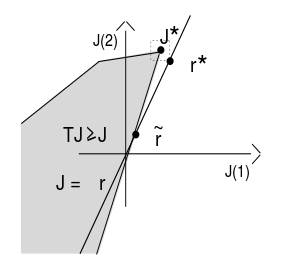
\includegraphics{FV_alp_proj.png}}
\caption{\label{fig:FV1} Graphical Representation of ALP, from de FArias and Van Roy \cite{FV}.}
\end{center}
\end{figure}

The figure \ref{fig:FV1} shows how the solution to the ALP $\tilde{r}$ does not necessarily yield an approximation, $\Phi\tilde{r}$, as good as $\Phi r^*$, the projection of $J^*$ onto the subspace spanned by the basis functions $\phi_i$. Our next bound shows how we can relate the solution of the approximate linear program to the ``best'' approximation in the space spanned by $\Phi$ -- $\Phi r^*$.

\begin{thm}\label{thm:alpbound2}
Let $e$ be in $\text{span}(\phi_1,\dots,\phi_k)$ and by $c$ denote a probability distribution on the state space. Then if $\tilde{r}$ is an optimal solution to the approximate linear program,
$$
||J^* - \Phi\tilde{r}||_{1,c} \leq \frac{2}{1-\alpha} \min_r || J^* - \Phi r||_{\infty}
$$
\end{thm}

Above, the notation $||J||_{\infty}$ signifies $\max_{x \in S} |J(x)|$. Theorem \ref{thm:alpbound2} is given in more general terms, but the notation is intentional as it maps directly onto the notation used throughout the exposition of the problem and results regarding it. The result is due to de Farias and Van Roy \cite{FV}.

de Farias and Van Roy proceed to develop an improved bound, which can be sharper, as the bound given in Theorem \ref{thm:alpbound} does not take into account state-relevnace weights and instead in order for that bound to be small, it must be the case that the approximation shows low error across all states. This improved bound incorporates a weighted norm of the errors across states, depending upon how they are weighted in solving the ALP. We do not discuss this bound here, but it is mentioned because its development - through use of Lyupanov functions - is quite similar to the bound developed in another paper for the reduced linear program, discussed in Section \ref{solve_alp:cs} \cite{FV2}.

\section{Reduced Linear Program -- Constraint Sampling} \label{solve_alp:cs}

To approximate the approximate linear program, we create a new program called the ``reduced'' linear program or RLP. To create a RLP we set a number of constraints $m$, and because each constraint in the approximate linear program can be uniquely identified by a state, action pair, we introduce a probability distribution on the pairs which we denote by $\phi$ -- the set of constraints will be denoted $\sL$, we will consider this to be a set indexing the constraints. We also introduce a set $\sN$ to bound the possible solutions to the RLP, that is $\sN \subset \R^K$. We then generate a set $D$ of state, action pairs by independently sampling the space of state, action pairs according to $\phi$.

Therefore the program that we wish to solve is
\begin{align*}
\text{maximize } & c^T \Phi r & \\
\text{subject to } & g_a(x) + \alpha \sum_{x' \in S} p_a(x,x')(\Phir)(y) \geq (\phi r) (x), & \forall (a,x) \in D \\
& r \in \sN & \\
\end{align*}

Denote an optimal solution to the relaxed linear program given above as $\hat{r}$. Our goal should not be to try to ensure that this solution be close to the optimal solution of the exact linear program -- such an effort is not possible because so much depends on the choice of basis functions -- but to ensure ``closeness'' of the solution to the optimal solution of the approximate linear program. Specifically the requirement is that
$$
Pr[ | ||J^* - \Phi\hat{r}||_{1,c} - ||J^* - \Phi \tilde{r}||_{1,c}| \leq \epsilon ] \geq 1 -\delta
$$
$\delta$ is a confidence level regarding the closeness of the error of the RLP solution to that of the ALP solution.

Because the solution to the relaxed linear program, as only some constraints are present, may not be a solution to the approximate linear program, we need to study two properties of using a reduced linear program
\begin{itemize}
\item Sample complexity of near-feasibility
\item Sample complexity of approximation quality
\end{itemize}

Specifically, it is relevant for us to study how these properties can be obtained with respect to sampling constraints. The intuition behind this method is that if $|\sL|$ is infinite or huge and finite, each individual constraint may be inactive or only marginally affect the feasible region. Thus we hope we can only consider a subset of the constraints in $\sL$ and acheive a solution for the original problem that is feasible and of reasonable quality.

\subsection{Complexity of Near Feasibility}
Define the feasibility condition as follows: consider a set of linear constraints of the form
$$
y_z^T r + k_z \geq 0, \forall z \in \sL
$$
where $\sL$ is a set of indices for the constraints and $r \in \R^k$. Next we introduce a probability measure $\psi$ on $\sL$, an error tolerance $\epsilon$ and a confidence level $1-\delta$. 

The role of the distribution $\psi$ is both to sample and to assess the resulting sample \cite{FV2}. Specifically, we use this error tolerance $\epsilon$ and $\psi$ to assess quality in the sense that we define our objective as finding a subset $W \subset \sL$ such that
$$
\sup_{\{r | y_z^Tr + k_z \geq 0, \forall z \in W\}} \psi(\{ z' | y_{z'}^T r + k_{z'}\}) \leq \epsilon
$$

When the condition regarding the subset $W$ is met, $W$ is said to lead to near-feasibility. Then Theorem \ref{thm:sample_complexity} can be proven, regarding the sample complexity of near feasibility \cite{FV2}.

\begin{thm}\label{thm:sample_complexity}
If we have any $\delta \in (0,1)$ and $\epsilon \in (0,1)$ and $m$ such that
$$
m \geq \frac{4}{\epsilon} (K \log \frac{12}{\epsilon} + \log \frac{2}{\delta})
$$
Then, a set of $m$ (possibly repeated) i.i.d. randoms draws according to $\psi$ from $\sL$, which we will call $W$, satisfies
$$
\sup_{\{r | y_z^Tr + k_z \geq 0, \forall z \in W\}} \psi(\{ z' | y_{z'}^T r + k_{z'}\}) \leq \epsilon
$$ 
with probability $1-\delta$.
\end{thm}

The above, in asymptotic terms, tells us that if we have a sample size on the order of
$$
m = O(\frac{1}{\epsilon}(K \log \frac{1}{\epsilon} + \log \frac{1}{\delta}))
$$
then with probability at least $1-\delta$ we have that there is a $X \subset \sL$ such that $\psi(X) \geq 1 - \epsilon$ where every vector satisfying the constrants in $W$ (our sample of size $m$) also satisfies all the constraints in $Z$. That is, our sample of size $m$, with probability $1- \delta$, is near feasible. This is a very useful gaurantee because it is {\em independent} of the number of the constraints, and requires no knowledge about their structure.

\subsection{Complexity of Approximation Quality}
First a type of function is introduced which will be crucial to proving a bound on the quality of approximation. For any function $V: S \rightarrow \R$ define the scalar
$$
\beta_V = \max_{x \in S} \frac{\alpha(P_{u^*}V)(x)}{V(x)}
$$
corresponding to some policy $u^*$, in this case the optimal policy. This scalar is a measure of the maximum ratio of the next expected value of a state as compared to the current value over the entire state space. If this is small it conveys some sense of stability of the values of $V(x)$ over our system.

Further we can define a family of probability distributions over $S$ for each policy $u$ where the probability of each state is proportional to the expected discounted number of visits given an initial disribution according to $c$ as given below
$$
\mu_u^T = (1-\alpha)c^T(I - \alpha P_u)^{-1}
$$

Next Van Roy and de Farias define, for each Lyapunov function $V$, a probability distribution over $S$
$$
\mu_{u,V}(x) = \frac{\mu_u(x)V(x)}{\mu_u^TV}
$$
a distribution over state,action pairs
$$
\psi_{u,V}(x,a) = \frac{\mu_{u,V}(x)}{|A_x|}
$$
a constant
$$A = \max_{x \in S} |A_x|$$
and a constant
$$\theta = \frac{1 + \beta_V}{2} \frac{\mu_{u^*}T V} { c^T J^*} \sup_{r \in N} ||J^* - \Phi r||_{\infty, 1/V}$$
It is easy to verify that the distributions defined are in fact probability distributions.

With these defined, we can now present de Farias and Van Roy's main result \cite{FV2}.

\begin{thm}
Consider $\epsilon$, $\delta$ in $(0,1)$. Let $u^*$ be an optimal policy and $W$ be a set of $m$ state, action pairs sampled according to $\psi_{u^*,V}$ for some Lyupanov function $V$, where
$$
m \geq \frac{16A\theta}{(1-\alpha)\epsilon} (K \log \frac{48 A\theta}{(1-\alpha)\epsilon} + \log \frac{2}{\delta})
$$
Let $\tilde{r}$ be an optimal solution of the approximate linear program such that $\tilde{r} \in \sN$, and allow $\hat{r}$ to be an optimal solution of the relaxed linear program. Then with probability at least $1-\delta$
$$
||J^* - \Phi \hat{r} ||_{1,c} \leq ||J^* - \Phi \tilde{r} ||_{1,c} + \epsilon ||J^*||_{1,c}
$$
\end{thm}

The important things to note in this bound are the dependence on $V$ and $\sN$. Choice of these in general requires some intuition regarding the optimal policy, but careful selection can clearly affect how well this bound performs. An application studied in the literature is queueing networks where using the methods above, if $V$ and $\sN$ are chosen properly, the number of constraints that must be sampled grows quadratically with respect to the state space \cite{FV2}. de Farias and Van Roy also show how to exchange complexity in terms of large action spaces for size in the state space -- this is undesirable as the sample size grows polynomially in the maximum number of actions available in some state.


\section{Applications}

In this section description of some problems suited to these methods are described, and  it is explained how they might be tackled within the framework given in the preceding sections.

\subsection{Application to Playing Tetris}

One application of interest to approximate dynamic programing is to playing the game of tetris. Tetris is a game played on a $16 \times 7$ board where each space either has a block or not. New blocks come in 7 different shapes, and must be placed into the grid one at a time. They must be supported by at least one block already in the grid. New blocks are chosen by the game at random to present the player. The player scores points by ``clearing'' a row, which means to fill it completely from one side to the other.

Tetris is an interesting stochastic control problem because it is easily to envision the interplay between policy and cost-to-go (score). Further, it has such a large state space that it would be futile to try to solve a dynamic program to find an optimal policy directly. Thus, approximate methods must be use and using our approach, we must choose appropriate basis functions. These are problem specific, and require a good deal of intuition. Just because we find some that yield a solution we are happy with, we still have no idea if these are the best basis functions we can find or if we can find better. Common basis functions for Tetris include
\begin{itemize}
\item Maximum height of the wall
\item Number of holes
\item Heights of individual columns
\item Heights of adjacent columns
\item The constant 1
\end{itemize}

All of the basis functions above make intuitive sense, but what about the constant 1? It allows for an offset in case that is helpful for modelling this problem - in modelling many problems . We do not perform simulations of these methods on tetris, as time did not permit, but provide this example to help illustrate the power of these methods. Empirical results from the literature are quite good -- use of approximate dynamic programming via the linear programming approach has yielded policies which perform as well, on average, as an expert human player.

\section{Saddle Point Problems}

A major class of problems that fall under the umbrella of optimzation is the solution of deterministic and stochastic Saddle Point Problems. We focus our work on primal \emph{Dual Methods} for a particular class of problems -- techniques which will later be applied to solution of approximate dynamic programming problems.
That is why we try to formulate Dynamic Programming problem in the framework of the optimisation methods we study.

The procedure is as follows: first we investigate the stochastic minmax problem presented in\cite{NemirovskiRubinstein}. Then continue to look at an \emph{accelerated method}, in both the deterministic \cite{ChambollePock} and stochastic case \cite{ChenLanOuyang}, with the goal of applying these methods to approximate dynamic programming via the solution of linear programming problems.

\subsection{Setting}

Given a function $\Phi$ we study the general problem (that we call this problem the Primal Problem):
$$
\boxed{ (P): \min_{x \in X}\max_{y \in Y} \Phi(x,y) }
$$

Under the two following assumptions:

\begin{itemize}
\item A)$X$ and $Y$ are convex, compact sets.\\ $\Phi$ is convex in the first variable, concave in the second variable and Lipschitz on $X \times Y$
\item B) $\Phi$ is not necessarily differentiable in each of its variables but $\partial_{x} \Phi(x,y) \neq  \emptyset $ and $\partial_{y} \Phi(x,y) \neq  \emptyset $
%$\nabla_{x}\Phi(x,z)$ and $\nabla_{x}\Phi(x,y)$ are not directly accessibles (THEY DO NOT NECCESSARILY EXIST)
 we only have access to $g_{x}$ and $g_{y}$ such that $\forall (x,y) \in X \times Y$: \\
$$\mathbb{E}[g_{x}(x,y)] \in \partial_{x} \Phi(x,y) $$
$$\mathbb{E}[g_{y}(x,y)] \in \partial_{y} \Phi(x,y) $$

Additionally, we suppose that:

$$
\mathcal{L} = D_{X} \sup_{(x,y) \in X \times Y} \sqrt{\mathbb{E}[\lVert g_{x}(x,y) \rVert^{2}]}+ D_{Y} \sup_{(x,y) \in X \times Y}\sqrt{\mathbb{E}[\lVert g_{y}(x,y) \rVert^{2}]} < \infty
$$

Where $D_{X}$ and $D_{Y}$ are the euclidian diameters of $X$ and $Y$.

\end{itemize}

The first problem is called the \text{primal} problem. We also define the \text{dual} problem

$$
(D): \max_{y \in Y}\min_{x \in X} \Phi(x,y)
$$

Under Assumption A), by the \emph{MinMax Theorem}, we have 

$$
\max_{y \in Y}\min_{x \in X} \Phi(x,y) = \min_{x \in X}\max_{y \in Y} \Phi(x,y)
$$

Looking for a solution of $(P)$ is equivalent to finding a solution of $(D)$.

Now if we define:
\begin{itemize}
\item $\overline{\Phi}(x) = \max_{y \in Y}\Phi(x,y)$
\item $\underline{\Phi}(y) = \min_{x \in X}\Phi(x,y)$
\end{itemize}



We can set set up  an accuracy measure:
$$
\boxed{ \varepsilon(x,y) = [\overline{\Phi}(x) - \min_{X}\overline{\Phi}] + [\max_{Y}\underline{\Phi} - \underline{\Phi}(y)] }
$$

Since $\min_{X}\overline{\Phi} = \max_{Y}\underline{\Phi}$ (by  strong duality) we have:
$$
\boxed{\varepsilon(x,y) = \overline{\Phi}(x) - \underline{\Phi}(y)}
$$

If $(x^{*},y^{*})$ are the solution of the primal problem $(P)$,
then $\forall x, y \in X \times Y$:
$$
\underline{\Phi}(y) \leq \Phi(x^{*},y^{*}) \leq \overline{\Phi}(x)
$$

With equality iff $x = x^{*}$ and $y = y^{*}$.

\subsection{Motivations}

We keep in mind one particular application.
In Dynamic Programming (DP), the solution of the Bellman equation
$$
V^{*}(s) = \max_{a \in \mathcal{A}} \{ R(s,a) + \gamma \sum_{s^{'} \in \mathcal{S}} \mathbb{P}(s^{'} | s,a)V^{*}(s^{'}) \}
$$

can be formulated under the form of a Linear Program.\\

Where:
\begin{itemize}
\item $\mathcal{A}$ the set of possible actions.
\item $\mathcal{S}$ the set of possible states.
\item $\mathbb{P}(s^{'} | s,a)$ is the probability of transition from $s$ to $s^{'}$ when the action a is chosen.
\end{itemize}



Indeed $V^{*}$ can be seen as a vector of $\mathbb{R}^{|\mathcal{S}|}$, and in that case the previous equation becomes:
\begin{equation}\label{MLSDP}
\begin{array}{cl}
\min_{V^{*} \in \mathbb{R}^{|\mathcal{S}|}} & \sum_{s} V^{*}(s)  \\
\text{s.t.} & \forall (s, a)\in \mathcal{S} \times \mathcal{A}, \hspace{0.1cm} V^{*}(s) \geq R(s,a) + \gamma \sum_{s^{'}}\mathbb{P}(s^{'}| s,a )V^{*}(s^{'})\\
\end{array}
\end{equation}

As every Linear Program, this problem can be reduced to the resolution of a Saddle point Problem via its Lagrangian:
$$
\min_{V^{*}}\max_{\lambda \geq 0}\{ \sum_{s} V^{*}(s) + \sum_{a,s}\lambda_{a,s}[R(s,a) + \gamma \sum_{s^{'}}\mathbb{P}(s^{'}| s,a )V^{*}(s^{'}) - V^{*}(s)] \}
$$
However, since the set of space and actions is usually extremely large, this Linear Program suffers from the curse of dimensionnality.

One way to overcome this issue is to consider that $V^{*}(s)$ can be approximated by a linear combination of basis function.

This approximation yields \emph{noise} in the value of all the functions and \emph{thus} yields noise in the approximation of the gradients.



\subsection{Algorithm: Stochastic Approximation for Saddle Point (SASP) Problems}

A first algorithm is proposed in \cite{NemirovskiRubinstein} to solve Saddle Point Problems


Let's define the following functions:
\begin{itemize}
\item $$\pi_{X \times Y}[x,y] = \begin{pmatrix} \arg\min_{u \in X}\lVert x - u \rVert_{2}^{2} \\ \arg\min_{v \in Y}\lVert y - v \rVert_{2}^{2} \end{pmatrix}$$

The projection on the product of the two sets $X$ and $Y$.

\item $$\psi(x,y;\omega) = \begin{pmatrix} \rho_{X} g_{x} \\ -\rho_{Y} g_{y}  \end{pmatrix}$$

Where $\rho_{X}$ and $\rho_{Y}$ are two \emph{adequately} chosen parameters.

\end{itemize}


\vspace{0.5cm}

Then the algorithm to solve the stochastic saddle point problem is simply:

\vspace{0.5cm}




\begin{itemize}
\item Pick $x_{0} \in X$ and $y_{0} \in Y$
\item $\begin{pmatrix} x_{t+1} \\ y_{t+1} \end{pmatrix} = \pi_{X \times Y}[\begin{pmatrix} x_{t} \\ y_{t} \end{pmatrix} - \gamma_{t}\psi(x_{t},y_{t};\omega)]$
\item Return 
$$
\begin{pmatrix} x^{t} \\ y^{t} \end{pmatrix} = \dfrac{1}{t - \tau_{*}(t) + 1}\sum_{\tau = \tau_{*}(t)}^{t}\begin{pmatrix} x_{\tau} \\ y_{\tau} \end{pmatrix}
$$
\end{itemize}


Of course this algorithm depends on some parameters. The choice of those parameters has an influence on the convergence of the algorithm. We analyse those parameter as well as the convergence of the algorithm below.

\subsection{Analysis of the Convergence}

\begin{thm}

Under assumptions A), B) and if we choose $\gamma_{t} = C.t^{-\alpha}$

Then

$$
\mathbb{E}[\varepsilon(x^{N},y^{N})] \leq [D_{X}^{2}\rho_{X}^{-1} + D_{y}^{2}\rho_{Y}^{-1}]\dfrac{N^{\alpha}}{C(N - \tau_{*}(N) + 1)} +  \dfrac{\mathcal{L}}{\sqrt{N - \tau_{*}(N) + 1}}+ C\mathcal{L}^{2}[\rho_{X}D_{X}^{-2} + \rho_{Y}D_{Y}^{-2}]\tau_{*}^{-\alpha}(N)
$$

\end{thm}


WE can notice that the previous rate of convergence results depends on the parameters. It seems therefore reasonable 
to optimise the parameters.

\begin{cor}
Optimizing over the prameters yields:
 $\rho_{X} = D_{X}^{2}$,
$\rho_{Y} = D_{Y}^{2}$,
$\tau_{*}(t) = \dfrac{t}{2}$,
$\alpha = \dfrac{1}{2}$,
$C = \dfrac{2}{\mathcal{L}}$,

Giving:
$$
\boxed{ \mathbb{E}[\varepsilon(x^{N},y^{N})]  \leq 10\mathcal{L} N^{-\frac{1}{2}} }
$$
\end{cor}


The previous result uses only fixed step sizes, i.e. the step sizes are not adapted at each iteration.
In fact, the same kind of results apply when the step sizes are updated at each iteration.

More particularly, if we add the assumption:

\begin{itemize}
\item C) For $t$, $C_{t}$ depends only on the observations collected at the first steps, i.e. 
$$C_{t} = f\big(g_{x}(x^{1},y^{1}),g_{y}(x^{1},y^{1}),...,g_{x}(x^{t-1},y^{t-1}),g_{y}(x^{t-1},y^{t-1})\big)$$
and 
$$
C_{*} \leq C_{t} \leq C^{*}
$$
Where $C_{*}$ and $C^{*}$ being two arbitrary constants,

\end{itemize}

then the following holds:

\begin{thm}
If assumptions $A)$, $B)$ and $C)$ hold and if we choose the step size in the SASP as $\gamma_{t} = C_{t}t^{-\alpha}$,
$\rho_{X} = D_{X}^{2}$, $\rho_{Y} = D_{Y}^{2}$ and $\tau^{*}(t) = \dfrac{t}{2}$, then:

\begin{align*}
\mathbb{E}[\varepsilon(x^{N},y^{N})] &\leq [D_{X}^{2}\rho_{X}^{-1} + D_{Y}^{2}\rho_{Y}^{-1} ][1 + \dfrac{1}{2C^{*}}\sum_{}^{N}\sup_{\tau \leq t} | C_{\tau} - C_{\tau-1}|]
[\dfrac{N^{\alpha}}{C_{*}(N - \tau_{*}(N) + 1)}] \\ 
&+ \dfrac{\mathcal{L}}{\sqrt{N - \tau_{*}(N)+ 1}} + \dfrac{C^{*}\mathcal{L}[\rho_{X}D_{X}^{-2} + \rho_{Y}D_{Y}^{-2}]}{\tau_{*}^{\alpha}(N)}
\end{align*}
\end{thm}


The proofs of Theorem 1 and 2 are somehow similar.
We give here a brief overview of those two proofs.

\begin{proof}

The main idea of the proof consists of defining a distance on $X \times Y$.
Then, after fixing $(x,y)\in X \times Y$, we define $d_{t} = d((x,y),(x_{t},y_{t}))$ the distance between $(x,y)$
and the output of the algorithm at time $t$.
By 1-lipschitziannity of the projection, and convexity of $\Phi$ in the first variable, we obtain a bound on:
$$
\Phi(x_{t},y) - \Phi(x,y_{t})
$$
$\forall t \leq N$.
By summing this bound over $t$, and applying Cauchy Inequality we now have a bound on
$$
\Phi(x_{N},y) - \Phi(x,y_{N})
$$

Considering the expectation and some additional computations later, we obtain the desired result.

\end{proof}

\subsection{Online version of the algorithm}

In our setting, to \emph{optimize} the parameters, we need to have access to some quantities dependent on the problem geometry of the constraints of the problem (e.g. $\mathcal{L}$, $D_{X}$ and $D_{Y}$).

For instance
$$
\mathcal{L} = D_{X} \sup_{(x,y) \in X \times Y} \sqrt{\mathbb{E}[\lVert g_{x}(x,y) \rVert_{2}^{2}]} + 
D_{Y} \sup_{(x,y) \in X \times Y} \sqrt{\mathbb{E}[\lVert g_{y}(x,y) \rVert_{2}^{2}]}
$$

cannot be computed exactly.
Therefore we approximate $\mathcal{L}$ with  
$$
L_{t} = D_{X}\sqrt{\dfrac{1}{t}\sum_{\tau=1}^{t}\kappa_{x}(\lVert g_{x}^{\tau} \rVert_{2})^{2}} + D_{Y}\sqrt{\dfrac{1}{t}\sum_{\tau=1}^{t}  \kappa_{y}(\lVert g_{y}^{\tau} \rVert_{2})^{2}}
$$

$\kappa_{x}$ and $\kappa_{y}$ are two truncation function.
(e.g. $\kappa_{s}(t) = A_{s}^{-}1_{ t < A_{s}^{-}}(t) + A_{s}^{+}1_{ t \geq A_{s}^{+}}(t) + t 1_{ [A_{s}^{-}, A_{s}^{+}]}(t)$).
We truncate the sample variances to avoid too large or too small fluctuations.
%
%$$
%\gamma_{t} = C_{t}t^{-\frac{1}{2}}
%$$
%$$
%C_{t} = \dfrac{2}{L_{t}}
%$$
%
%With 
%$$
%L_{t} = D_{X}\sqrt{\dfrac{1}{t}\sum_{\tau=1}^{t}\lVert g_{x}^{\tau} \rVert_{2}^{2}} + D_{Y}\sqrt{\dfrac{1}{t}\sum_{\tau=1}^{t}  \lVert g_{y}^{\tau} \rVert_{2}^{2}}
%$$

%\subsection{Discussion on the algorithm}

\subsection{Numerical results}

We consider the somehow standard min max problem:
$$
\min_{x}\max_{y} f_{s}(x,y)
$$
with $f_{s}(x,y) = (1 - 2y)(x - s) + \dfrac{1}{2}(x - s)^{2} - \dfrac{1}{2}s^{2} $

We have 

\begin{itemize}
\item $\partial_{x} f_{s}(x,y) = 1 - 2y + x - s$
\item $\partial_{y} f_{s}(x,y) = -2x + 2s$
\end{itemize}

The addition of noise gives

\begin{itemize}
\item $g_{x} f_{s}(x,y) = 1 - 2y + x - s - \omega$
\item $g_{y} f_{s}(x,y) = -2x + 2s + 2\omega$
\end{itemize}

with $\omega \sim \mathcal{N}(0,1)$

\section{ A specific Example of Saddle Point Problem}

We now consider a particular  non smooth saddle point problem.

\subsection{Introduction}

In many applications, particularly imaging some saddle point problem occur. The following problem is a good example of such a problem.
If we define:
$$
f(x) = \max_{y \in Y} \{ G(x) + (Kx,y) - J(y) \} 
$$
and if we seek the minimum of the of $f$ over the set $X$, then the optimisation problem transforms to a saddle point problem.
\begin{align*}
\min_{x \in X} f(x) &= \min_{x \in X}\max_{y \in Y} \{ G(x) + (Kx,y) - J(y)\} \\
&= \min_{x \in X} (G(x) + \max_{y \in Y} \{  (Kx,y) - J(y)\})\\
&= \min_{x \in X} (G(x) + J^{*}(Kx)) \numberthis \label{SPPpart}
\end{align*}
where $J^{*}$ is the Fenchel conjugate of $J$.

We suppose that G is strongly convex, i.e. that:
$$
G(y) - G(x) - \langle \nabla G(x),y - x\rangle \leq \dfrac{L_{G}}{2} \lVert x - y \rVert_{2}^{2}
$$
This implies that strong duality holds (assumption A) holds).
$$
\min_{x \in X}\max_{y \in Y} \{ G(x) + (Kx,y) - J(y)\} = \min_{x \in X}\max_{y \in Y}\min_{x \in X} \{ G(x) + (Kx,y) - J(y)\}
$$

Several Primal Dual algorithms have been derived on this subject.
We give a brief summary of the results below.

We distinguish 

\begin{itemize}
\item the \emph{Deterministic} case: some values of the sub gradients are available
\item the \emph{Stochastic} case:  some noisy values of the sub gradients are available. 
The expected values being the actual sub gradients.
\end{itemize}

\subsection{Motivation}

Now if we still consider the case of the LP associated to the resolution of Dynamic Programming,
we have to solve the following saddle point problem

$$
\min_{V^{*}}\max_{\lambda \geq 0}\{ \sum_{s} V^{*}(s) + \sum_{a,s}\lambda_{a,s}[R(s,a) + \gamma \sum_{s^{'}}\mathbb{P}(s^{'}| s,a )V^{*}(s^{'}) - V^{*}(s)] \}
$$

This problem can exactly be written in the previous form.


With 

\begin{itemize}
\item First we can notice that the set of $(V^{*}(s))_{s \in \mathcal{S}}$ 
can be seen as a a vector of $\mathbb{R}^{\mathcal{S}}$. In this case we can define
$$G(V^{*}) = 1^{T}V^{*} = \sum_{s} V^{*}(s)$$
\item The second term 
$$
\sum_{a,s}\lambda_{a,s}[R(s,a) + \gamma \sum_{s^{'}}\mathbb{P}(s^{'}| s,a )V^{*}(s^{'}) - V^{*}(s)]
$$
can be seen as a scalar product between $(\lambda)_{a,s}$ and $(R(s,a) + \gamma \sum_{s^{'}}\mathbb{P}(s^{'}| s,a )V^{*}(s^{'}) - V^{*}(s))_{a,s}$.

\end{itemize}

\subsection{ Review of the results on Saddle Points Problems: }


In this section, we propose a review of the optimisation algorithms existing to solve problem \ref{SPPpart}, in both the deterministic and the stochastic case.

\subsubsection{Deterministic SPP: }



\begin{itemize}

\item By non smoothness of the objective function in general, applying a classic sub gradient method \cite{YudinNemirovski} yield a rate of convergence of
$$
O(\dfrac{1}{\sqrt{N}})
$$

\item In \cite{Nesterov}, Nesterov proposes to approximate the objective function by a smooth function and then apply an accelerated gradient method yielding, assuming that $X$ and $Y$ are compact, a rate of convergence of:
$$
O(\dfrac{L_{G}}{N^2} + \dfrac{L_{K}}{N})
$$

\item In \cite{ChambollePock}, a Primal Dual Method is proposed that achieves the following convergence rate:
$$
O(\dfrac{L_{G} + L_{K}}{N})
$$
\item A method achieving the optimal rate of convergence consists of an accelerated version of the primal dual method developed in \cite{ChenLanOuyang}.
Moreover, this method is shown to work in the case where $X$ and $Y$ are non bounded.
The obtained rate of convergence is:

$$
O(\dfrac{L_{G}}{N^2} + \dfrac{L_{K}}{N})
$$


\end{itemize}

In the following, we focus on the last method, achieving the optimal convergence rate.

%
%In \cite{ChenLanOuyang}, an Accelerated Primal Dual (APD) algorithm is proposed, that achieves such a bound (in the deterministic case).




\subsubsection{ Stochastic SPP: }

A lower bound on the rate of convergence of Stochastic Programming is shown in \cite{YudinNemirovski} to be

$$
O(\dfrac{L_{G}}{N^{2}} + \dfrac{L_{K}}{N}  + \dfrac{\sigma_{x} + \sigma_{y}}{\sqrt{N}})
$$

Below we briefly review some the rate of convergence of some stochastic approximation algorithms.

\begin{itemize}
\item Mirror descent stochastic Approximation (MDSA): This is basically the method we presented in the first section.

$$
O((L_{G} + L_{K} + \sigma_{x} + \sigma_{y})\dfrac{1}{\sqrt{N}})
$$

\item Stochastic Mirror Prox (SMP) an improvement of the method described in the first section yields a rate of convergence of:

$$
O(\dfrac{L_{G} + L_{K}}{N} + \dfrac{\sigma_{x} + \sigma_{y}}{\sqrt{N}})
$$

\item Accelerated Stochastic Approximation (AC-SA) is a stochastic version of Nesterov's method that achieves the following convergence rate:

$$
O(\dfrac{L_{G}}{N^{2}}) + (L_{K} + \sigma_{x} + \sigma_{y})\dfrac{1}{\sqrt{N}}
$$
\end{itemize}

In \cite{ChenLanOuyang}, a stochastic version of the APD method is proposed that achieves the lower bound on the rate 
of convergence
$$
O(\dfrac{L_{G}}{N^{2}} + \dfrac{L_{K}}{N} + \dfrac{\sigma_{x} + \sigma_{y}}{\sqrt{N}})
$$

%\subsection{Contribution of the paper: }
%
%\begin{itemize}
%\item Accelerated Primal Dual (APD) method for deterministic SPP.\\
%Idea: add a multi-step acceleration scheme into the primal dual method
%Rates of convergence: optimal $O(\dfrac{L_{G}}{N^{2}} + \dfrac{L_{K}}{N})$
%\item Stochastic version of APD method.\\
%Achieves the lower bound on the rate of convergence
%$$
%O(\dfrac{L_{G}}{N^{2}} + \dfrac{L_{K}}{N} + \dfrac{\sigma_{x} + \sigma_{y}}{\sqrt{N}})
%$$
%\item For both deterministic and stochastic SPP, the developed APD algorithms can deal with unbounded $X$ and $Y$ (as long as the saddle point problem exists). 
%\end{itemize}

\section{Study of a particular algorithm: Primal Dual algorithm to solve the problem: }

\subsection{Algorithm}


This algorithm has been proposed  by Chambolle and Pock in \cite{ChambollePock}

\begin{itemize}
\item $x_{1} \in X$, $y_{1} \in Y$. Set $\overline{x}_{1} = x_{1}$
\item

\begin{itemize}
\item $y_{t+1} = \arg\min_{y \in Y} (-K\overline{x}_{t},y) + J(y) + \dfrac{1}{2\eta_{t}} \lVert y - y_{t} \rVert_{2}^{2}$
\item $x_{t+1} = \arg\min_{x \in X} G(x) + (Kx,y_{t+1}) + \dfrac{1}{2\eta_{t}}\lVert x - x_{t} \rVert_{2}^{2} $
\item $\overline{x}_{t+1} = \theta_{t}(x_{t+1} - x_{t}) + x_{t+1}$
\end{itemize}

\item $x^{N} = \dfrac{1}{N}\sum_{t=1}^{N} x_{t}$ and $y^{N} = \dfrac{1}{N}\sum_{t=1}^{N} y_{t}$
\end{itemize}

The stochastic method for saddle point problem we present below achieves the (almost) optimal rate of convergence 

\subsection{ Analysis of the algorithm: }


Although a good start for our problem, this algorithm is ineffective for solving the saddle point problem resulting in
the approximation of the resolution of Dynamic Programming.
Indeed, it requires the exact gradient. Moreover, the proof of convergence only holds if X and Y are bounded sets, which is not the case
of the saddle point problem induced by Lagrangian of the approximation of LP...

\section{ Accelerated Primal Dual Algorithm: }


Sometimes the step $x_{t+1} = \arg\min_{x \in X} G(x) + (Kx,y_{t+1}) + \dfrac{1}{2\eta_{t}}\lVert x - x_{t} \rVert_{2}^{2}$ can be hard to compute.
($G$ can be a "blackbox" function).

Locally (around $x_{t}$) $G$ can be approximated by:
$$
G(x) \approx G(x_{t}) + (\nabla G(x_{t}),x - x_{t})
$$

and the previous step becomes:

$x_{t+1} = \arg\min_{x \in X} (\nabla G(x_{t}),x) + (Kx,y_{t+1}) + \dfrac{1}{2\eta_{t}}\lVert x - x_{t} \rVert_{2}^{2}$

Moreover, instead of penalising by a Euclidian quadratic term, the penalisation can be generalised with a Bregman Divergence

\begin{itemize}
\item $V_{X}(x,u) = d_{X}(x) -  d_{X}(u) - \langle \nabla d_{X}(u),x - u \rangle$
\item $V_{Y}(y,v) = d_{Y}(y) -  d_{Y}(v) - \langle \nabla d_{Y}(v),y - v \rangle$
\end{itemize}

We can notice that with $d_{X}(x) = \lVert x \rVert_{2}^{2}$ and $d_{Y}(x) = \lVert y \rVert_{2}^{2}$ we obtain exactly the same term.

\subsection{Accelerated Primal Dual for Stochastic Saddle Point Problems:}

\begin{itemize}
\item choose $x_{1} \in X, y_{1} \in Y$. Set $\overline{x}_{1} = x_{1}$
\item

\begin{itemize}
\item $x_{t}^{md} = (1 - \dfrac{1}{\beta_{t}})x_{t}^{ag} +  \dfrac{1}{\beta_{t}}x_{t}$
\item $y_{t+1} = \arg\min_{y \in Y} \langle -K\overline{x}_{t},y\rangle + J(y) + \dfrac{1}{\tau_{t}}V_{Y}(y,y_{t})$
\item $x_{t+1} = \arg\min_{x \in X} \langle \nabla G(x_{t}^{md}) ,x \rangle + \langle x,K^{T}y_{t+1} \rangle + \dfrac{1}{\eta_{t}}V_{X}(x,x_{t})$
\item $x_{t+1}^{ag} = (1 -  \dfrac{1}{\beta_{t}})x_{t+1}x_{t}^{ag}+ \dfrac{1}{\beta_{t}}x_{t+1}$
\item $y_{t+1}^{ag} = (1 -  \dfrac{1}{\beta_{t}})y_{t+1}x_{t}^{ag}+ \dfrac{1}{\beta_{t}}y_{t+1}$
\item $\overline{x}_{t+1} = \theta_{t+1}(x_{t+1} - x_{t}) + x_{t+1}$
\end{itemize}

\item Output $x_{N}^{ag}$ and $y_{N}^{ag}$
\end{itemize}

\subsection{Analysis of the Algorithm}

\begin{thm}


If

\begin{itemize}
\item $\sup_{x_{1},x_{2}} V_{X}(x_{1},x_{2}) \leq \Omega_{X}^{2}$
\item $\sup_{y_{1},y_{2}} V_{X}(y_{1},y_{2}) \leq \Omega_{Y}^{2}$
\end{itemize}

and the parameters are chosen such that:

\begin{itemize}
\item $\beta_{1} = 1$, $\beta_{t+1} - 1 = \beta_{t}\theta_{t+1}$
\item $0 < \theta_{t} \leq \min\{ \dfrac{\eta_{t-1}}{\eta_{t}}, \dfrac{\tau_{t-1}}{\tau_{t}}\}$
\item $\dfrac{\alpha_{X}}{\eta_{t}} - \dfrac{L_{G}}{\beta_{t}} - \dfrac{L_{K}^{2}\tau_{t}}{\alpha_{Y}} \geq 0$
\end{itemize}

Then:
$$
g(z_{t+1}^{ag}) \leq \dfrac{1}{\beta_{t}\eta_{t}}\Omega_{X}^{2} + \dfrac{1}{\beta_{t}\tau_{t}}\Omega_{Y}^{2}
$$


\end{thm}

\begin{proof}

\end{proof}

\section{Stochastic APD}

In this setting we consider that we do not have access directly to $\nabla G(x)$ and to $Kx$ and $Ky$, but to some biased/noised values that we are going to call

$\mathcal{G}(x)$, $\mathcal{K}_{x}(x)$ and $\mathcal{K}_{y}(y)$.

We have $\mathcal{G}(x) = \nabla G(x) + \varepsilon_{g}$, $\mathcal{K}_{x}(x) = Kx + \varepsilon_{x}$, $\mathcal{K}_{y}(y) = Ky + \varepsilon_{y}$.

$\varepsilon_{g}$, $\varepsilon_{x}$ and $\varepsilon_{y}$ represent the (stochastic) zero means errors.


\begin{itemize}


\item (A1) $$\mathbb{E}[\lVert \mathcal{G}(x) - \nabla G(x) \rVert_{2}^{2}] \leq \sigma_{G}^{2}$$,

$$\mathbb{E}[\lVert \mathcal{K}_{x}(x) - Kx \rVert_{2}^{2}] \leq \sigma_{x}^{2}$$

$$\mathbb{E}[\lVert \mathcal{K}_{y}(y) - Ky \rVert_{2}^{2}] \leq \sigma_{y}^{2}$$

\item (A2) $$\mathbb{E}[\exp(\frac{\lVert \mathcal{G}(x) - \nabla G(x) \rVert_{2}^{2}}{\sigma_{G}^{2}})] \leq \exp{1}$$,

$$\mathbb{E}\exp(\frac{[\lVert \mathcal{K}_{x}(x) - Kx \rVert_{2}^{2}}{\sigma_{x}^{2}})] \leq \exp{1}$$

$$\mathbb{E}[\exp(\dfrac{\lVert \mathcal{K}_{y}(y) - Ky \rVert_{2}^{2}}{\sigma_{y}^{2}})] \leq \sigma_{y}^{2}$$
\end{itemize}


\section{Applying Saddle Point Methods to the Approximate Linear Program}

The main innovation of this project is to apply the aforementioned saddle point methods to solving approximate dynamic programs. Specifically, we perform our analysis in the context of solving approximate and reduced linear programs and then study how well these approximate optimal solutions and the rate of convergence.

[ TODO ]

\section{Conclusions and Future Directions}



[ TODO ]

\section{Partner Work and Contributions}

Carson was responsible for the linear programming approach to dynamic programing, its approximations and applications to specific problems. Thomas was responsible for studying and reporting on saddle point methods. Both partners contributed equally to the effort to combine results and to compile the seperate reports into a cohesive whole. Both partners participated in creating simulations, developing proofs and editing the final, submitted product.

% \subsection{An Algorithm}

% \subsection{Introducing Constraint Sampling}

% In the approximate LP, though there are fewer variables than in the original problem, there are as many constraints. 

% note the form of the bibliography. start with a bibitem.
% you refer to an entry in the bibliography by using the label in braces
% the computer prints the label in brackets. often I have both the same, but
% you don't have to.

\bibliographystyle{plain}
\bibliography{references}


\bigskip

\end{document}
